\documentclass[11pt,a4paper]{article}

% ---- Packages -------------------------------------------------------------
\usepackage[utf8]{inputenc}
\usepackage[T1]{fontenc}
\usepackage[margin=1in]{geometry}
\usepackage{array}
\usepackage{longtable}
\usepackage{xcolor}
\usepackage{listings}
\usepackage{enumitem}
\usepackage{titlesec}
\usepackage{tikz}
\usetikzlibrary{positioning, arrows.meta, calc}
\usepackage{adjustbox}
\usepackage[hidelinks]{hyperref}

% ---- Listings style (for code / register procedures) ----------------------
\definecolor{codebg}{rgb}{0.96,0.96,0.96}
\lstset{
  basicstyle=\ttfamily\small,
  backgroundcolor=\color{codebg},
  frame=single,
  breaklines=true,
  columns=fullflexible,
  keepspaces=true,
  showstringspaces=false,
}

% ---- TikZ styles for the architecture diagrams ----------------------------
\tikzset{
  blk/.style = {draw, semithick, rounded corners, align=center, font=\small,
                minimum height=10mm, inner xsep=3mm},
  ext/.style = {draw, semithick, dashed, rounded corners, align=center, font=\small,
                minimum height=10mm, inner xsep=3mm, fill=black!4},
  fwd/.style = {-{Latex[length=2mm,width=2mm]}, semithick},
  bi/.style  = {{Latex[length=2mm]}-{Latex[length=2mm]}, semithick},
  lbl/.style = {font=\scriptsize\ttfamily, inner sep=1.5pt, align=center},
}

\newcommand{\reg}[1]{\texttt{#1}}
\newcommand{\bit}[1]{\texttt{#1}}

\title{\textbf{Crypto Core --- Design \& Host Programming Manual}\\[4pt]
       \large Switchable AES-128 \textbf{CTR / CMAC / CCM} crypto-DMA accelerator with an
       AXI4-Lite control plane and an AXI4 master data plane}
\author{}
\date{}

\begin{document}
\maketitle

\noindent
This document describes (1) what the core does as a whole, (2) the role and internal
operation of every module, (3) the \textbf{data byte-order conventions} the host must follow,
and (4) how a host (software/CPU) drives the core --- the register map, the meaning of every
control/status bit, and a step-by-step operating procedure \emph{per mode}.

\medskip
\noindent\textbf{Status at a glance.} The core is a working, switchable multi-mode AES
accelerator. A single AES-128 engine is shared by three modes selected at run time by the
host: \textbf{CTR} (confidentiality), \textbf{CMAC} (authentication), and \textbf{CCM}
(authenticated encryption, both directions). All modes stream over the DMA data plane and
support whole-block and word-aligned partial payloads. The integration testbench
\texttt{tb\_cryptoCore\_dma} passes 34/34.

\tableofcontents
\bigskip

% ===========================================================================
\section{Overview --- what the core does}

The crypto core is the ``Crypto-Core (RUB)'' accelerator block of a larger SoC built around
an AXI crossbar. Like every accelerator in that system it has \textbf{two interfaces}:

\begin{itemize}[nosep]
  \item \textbf{REG-IF --- AXI4-Lite slave (control plane).} The host configures the core
        through a register file: select the mode and key, set the nonce/IV, program a
        transfer, start it, and poll status / read the result tag.
  \item \textbf{DATA-IF --- AXI4 full master (data plane).} The core \textbf{autonomously
        reads source data and writes results} to/from memory over the crossbar --- a
        ``crypto-DMA.'' The host hands the core a source address, a destination address, and a
        length; it does \emph{not} shuttle data block-by-block.
\end{itemize}

\subsection{The three modes (plus bypass)}
A 2-bit \bit{CTRL.MODE} field selects which cryptographic function the shared AES engine
performs for a given transfer:

\begin{longtable}{@{}p{0.10\textwidth} p{0.14\textwidth} p{0.66\textwidth}@{}}
\hline
\textbf{MODE} & \textbf{Function} & \textbf{What it does / produces} \\ \hline \endhead
\texttt{0} & \textbf{CTR}  & AES-128 Counter mode. Confidentiality only. Encrypt = decrypt
  (keystream XOR). Streams ciphertext (or recovered plaintext) to \reg{DST\_ADDR}. \\ \hline
\texttt{1} & \textbf{CMAC} & AES-CMAC (NIST SP 800-38B / RFC 4493). Authentication only ---
  reads the message, produces a 128-bit \textbf{tag} in \reg{TAG\_OUT}. No data is written
  back (read-only DMA). \\ \hline
\texttt{2} & \textbf{CCM}  & AES-CCM (NIST SP 800-38C). Authenticated encryption. Encrypt
  (\bit{DECRYPT}=0): writes ciphertext to \reg{DST\_ADDR} and the encrypted tag \(U\) to
  \reg{TAG\_OUT}. Decrypt+verify (\bit{DECRYPT}=1): writes recovered plaintext and sets
  \bit{STATUS.AUTH\_OK}. \\ \hline
\end{longtable}

\noindent In addition, \bit{CTRL.BYPASS} turns the path into a plain memory-to-memory copy
(no crypto). Bypass and the CTR/CMAC/CCM modes are mutually exclusive per transfer.

\paragraph{Shared AES engine.} There is exactly \textbf{one} AES-128 engine. A small
combinational arbiter (\reg{aesArbiter}) routes the engine's inputs to the controller for the
active mode (the CTR FSM, \reg{cmacEngine}, or \reg{ccmEngine}); the engine's outputs are
broadcast to all three. This keeps area low --- adding CMAC/CCM cost mostly control logic, not
a second cipher. \textbf{All three modes use AES encryption only} (CCM/CTR decryption is XOR
against forward-generated keystream), so no inverse cipher is needed.

\paragraph{Key properties.}
\begin{itemize}[nosep]
  \item \textbf{Algorithm:} AES-128. CTR counter block = \texttt{IV(96) || counter(32)};
        CMAC per RFC 4493; CCM per SP 800-38C with parameters \(q\)=2 (13-byte nonce),
        \(\text{Tlen}\)=16 (full tag), \textbf{no AAD} (current scope).
  \item \textbf{Crypto-DMA:} one AXI4 master port streams
        \texttt{read $\rightarrow$ engine $\rightarrow$ (write)}. The data path is 32 bits
        wide; the stream adapter gathers four 32-bit beats into each 128-bit block and
        scatters results back out.
  \item \textbf{Partial payloads:} whole-block \emph{and} word-aligned partial lengths
        (multiples of 4 bytes) are supported. Sub-word tails (arbitrary byte length) are not
        yet supported (see \S\ref{sec:limits}).
  \item \textbf{Two key slots:} \reg{key1}/\reg{key2}, selectable per transfer via
        \bit{CTRL.KEY\_SEL}; provisioned at boot (\texttt{BOOT\_ENABLE}=1) or loaded from the
        fixed test keys \texttt{STATIC\_KEY1/2} after reset (\texttt{BOOT\_ENABLE}=0, default),
        see below.
  \item \textbf{Nonce-uniqueness (CTR):} 96-bit host IV + 32-bit hardware counter that
        auto-increments per block and cannot roll back; a pre-flight gate refuses a transfer
        that would exhaust the per-IV counter budget or select an unloaded key.
  \item \textbf{Hardening:} keys are never readable over either bus and async-zeroize on reset.
\end{itemize}

\paragraph{Boot / key provisioning.}
Keys are provisioned at boot: on reset, \reg{bootCtrl} runs a fixed sequence that
DMA-fetches an encrypted bitstream, decrypts it on the shared AES, and writes the recovered
keys into \reg{keyStorage}. During boot, \bit{boot\_active} forces the arbiter to CTR and
gates the host register writes; \bit{STATUS.BOOT\_DONE} rises when provisioning completes.
\textbf{The host must wait for \bit{BOOT\_DONE} before configuring a transfer.} Boot details
are in \texttt{boot\_path\_spec.md}.

The boot sequence is enabled by the top-level parameter \textbf{\texttt{BOOT\_ENABLE}}
(default \textbf{0}). With \texttt{BOOT\_ENABLE}=1, \reg{bootCtrl} runs the sequence above.
With \texttt{BOOT\_ENABLE}=0 there is no boot and \textbf{no DATA-IF access after reset};
\bit{BOOT\_DONE} is 1 immediately, and one clock after reset \reg{key1}/\reg{key2} are loaded
from the parameters \texttt{STATIC\_KEY1} (default NIST SP~800-38A key \texttt{2b7e1516\ldots})
and \texttt{STATIC\_KEY2} (default FIPS-197 C.1 key \texttt{00010203\ldots}). These are
\textbf{public test keys}: there is no confidentiality, and ``keys zeroize on reset'' only holds
until the first clock after reset.

\paragraph{Architecture --- control plane (REG-IF).}
\begin{center}
\begin{adjustbox}{max width=\textwidth}
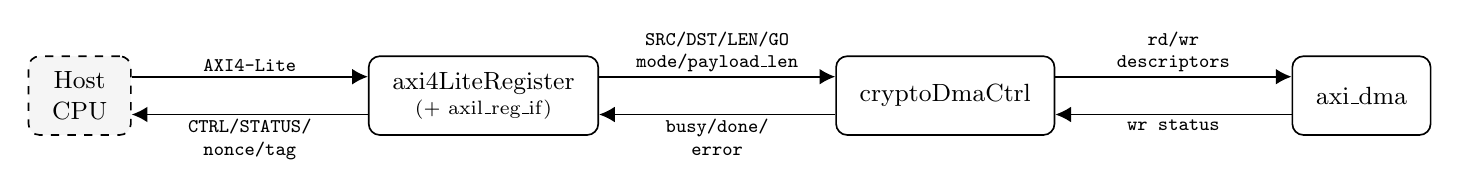
\begin{tikzpicture}[node distance=16mm and 30mm]
  \node[ext] (host) {Host\\CPU};
  \node[blk, right=of host] (regs) {axi4LiteRegister\\[-2pt]{\scriptsize(+ axil\_reg\_if)}};
  \node[blk, right=of regs] (dctl) {cryptoDmaCtrl};
  \node[blk, right=of dctl] (dma)  {axi\_dma};

  \draw[fwd] ([yshift=2.4mm]host.east) -- node[lbl,above]{AXI4-Lite} ([yshift=2.4mm]regs.west);
  \draw[fwd] ([yshift=-2.4mm]regs.west) -- node[lbl,below]{CTRL/STATUS/\\nonce/tag} ([yshift=-2.4mm]host.east);

  \draw[fwd] ([yshift=2.4mm]regs.east) -- node[lbl,above]{SRC/DST/LEN/GO\\mode/payload\_len} ([yshift=2.4mm]dctl.west);
  \draw[fwd] ([yshift=-2.4mm]dctl.west) -- node[lbl,below]{busy/done/\\error} ([yshift=-2.4mm]regs.east);

  \draw[fwd] ([yshift=2.4mm]dctl.east) -- node[lbl,above]{rd/wr\\descriptors} ([yshift=2.4mm]dma.west);
  \draw[fwd] ([yshift=-2.4mm]dma.west) -- node[lbl,below]{wr status} ([yshift=-2.4mm]dctl.east);
\end{tikzpicture}
\end{adjustbox}
\end{center}

\paragraph{Architecture --- data plane (DATA-IF), the crypto-DMA pipeline.}
\begin{center}
\begin{adjustbox}{max width=\textwidth}
\begin{tikzpicture}[node distance=14mm and 22mm]
  \node[ext] (mem) {Memory\\[-2pt]{\scriptsize(crossbar)}};
  \node[blk, right=of mem] (dma) {axi\_dma\\[-2pt]{\scriptsize AXI4 master}};
  \node[blk, right=of dma] (ad)  {aesStreamAdapter\\[-2pt]{\scriptsize AXIS $\leftrightarrow$ blocks}};
  \node[blk, below=of ad]  (eng) {mode engines\\[-2pt]{\scriptsize cryptoCoreFSM (CTR)\\ cmacEngine\\ ccmEngine}};
  \node[blk, right=of eng] (arb) {aesArbiter\\[-2pt]{\scriptsize mode mux}};
  \node[blk, right=of arb] (aes) {AES128\\engine};
  \node[blk, below=of eng] (ks)  {keyStorage\\[-2pt]{\scriptsize key1/key2 + valid}};

  \draw[bi] (mem.east) -- node[lbl,above]{AXI4\\bursts} (dma.west);
  \draw[fwd] ([yshift=2.4mm]dma.east) -- node[lbl,above]{read\\stream} ([yshift=2.4mm]ad.west);
  \draw[fwd] ([yshift=-2.4mm]ad.west) -- node[lbl,below]{write\\stream} ([yshift=-2.4mm]dma.east);

  \draw[fwd] (ad.south) -- node[lbl,right]{block feed /\\result} (eng.north);

  \draw[fwd] ([yshift=2.4mm]eng.east) -- node[lbl,above]{io\_key,\\io\_dataIn} ([yshift=2.4mm]arb.west);
  \draw[fwd] ([yshift=2.4mm]arb.east) -- node[lbl,above]{selected} ([yshift=2.4mm]aes.west);
  \draw[fwd] ([yshift=-2.4mm]aes.west) to[out=200,in=-20] node[lbl,below]{io\_dataOut (broadcast)} ([yshift=-2.4mm]eng.east);

  \draw[fwd] (ks.north) -- node[lbl,right]{key\_out} (eng.south);
\end{tikzpicture}
\end{adjustbox}
\end{center}
The \reg{aesStreamAdapter} gathers 128-bit blocks from the read stream and feeds the active
engine; for CTR/CCM it scatters the engine's output block to the write stream; for CMAC it
writes nothing (the tag goes to a register). In \textbf{bypass} it routes each read beat
straight to the write beat.

% ===========================================================================
\section{Module reference}

\subsection{\texttt{cryptoCore} --- top level (rtl/cryptoCore.v)}
The top-level wrapper. It exposes the AXI4-Lite slave (REG-IF) and AXI4 master (DATA-IF)
ports and wires the sub-modules together. Parameters (\texttt{AXI\_DATA\_WIDTH}=32,
\texttt{AXI\_ADDR\_WIDTH}=16, \texttt{AXI\_ID\_WIDTH}=8, \texttt{LEN\_WIDTH}=20) let the data
plane match the system bus; the 32/16 defaults are placeholders pending the crossbar widths.
\texttt{BOOT\_ENABLE} (default 0) enables the boot sequence; \texttt{STATIC\_KEY1/2} are the
keys loaded after reset when it is disabled (see \emph{Boot / key provisioning}).
Glue logic:
\begin{itemize}[nosep]
  \item \textbf{Decode CTRL:} \texttt{key\_sel=CTRL[0]}, \texttt{bypass=CTRL[1]},
        \texttt{mode=CTRL[3:2]}, \texttt{decrypt=CTRL[4]}. Boot forces the effective mode to
        CTR: \texttt{eff\_mode = boot\_active ? CTR : mode}.
  \item \textbf{Assemble STATUS} (8 bits, see \S\ref{sec:status}).
  \item \textbf{Instantiate} \reg{aesArbiter}, \reg{cmacEngine}, \reg{ccmEngine} alongside the
        CTR FSM; all four share the one AES engine through the arbiter.
  \item \textbf{Message start / result latch:} generates a one-cycle \texttt{eng\_start} (rising
        edge of \texttt{dma\_busy} in an engine mode) routed to the selected engine; latches the
        engine's \texttt{tag}/\texttt{auth\_ok} into \reg{TAG\_OUT}/\bit{STATUS} at completion
        and holds them until the next start.
  \item \textbf{read\_only / length:} CMAC sets \texttt{read\_only} (no write DMA); engine modes
        use \texttt{payload\_len} for the DMA byte-length (CTR uses \texttt{DMA\_BLOCKS<<4}).
\end{itemize}

\subsection{\texttt{aesArbiter} --- shared-AES mode mux (rtl/aesArbiter.v)}
A purely combinational 3:1 mux. It selects the AES inputs
(\texttt{io\_key}/\texttt{io\_dataIn}/\texttt{fsm\_enable}) from the CTR FSM, \reg{cmacEngine},
or \reg{ccmEngine} according to \texttt{eff\_mode}; the AES \emph{outputs} are wired to all
three engines directly (an idle engine ignores them). \textbf{\texttt{boot\_active} forces the
CTR master}, so bitstream boot always owns the engine regardless of the \bit{MODE} field.

\subsection{\texttt{cmacEngine} --- AES-CMAC controller (rtl/cmacEngine.v)}
Computes a 128-bit CMAC over the streamed message. Derives subkeys \(K_1,K_2\) from
\(L=\mathrm{AES}_K(0)\) (GF(\(2^{128}\)) doubling, \texttt{Rb}=0x87), runs the CBC-MAC chain
\(C_i=\mathrm{AES}_K(C_{i-1}\oplus M_i)\), and XORs the final block with \(K_1\) (complete last
block) or \(K_2\) (zero-padded partial block). Block interface:
\texttt{block\_in/valid/last/nbytes/ready}; result on \texttt{tag}/\texttt{tag\_valid}. Drives
the AES via the shared handshake. Validated standalone against all RFC 4493 test vectors.

\subsection{\texttt{ccmEngine} --- AES-CCM controller (rtl/ccmEngine.v)}
Authenticated encryption/decryption. Builds the CCM formatting block \(B_0\) (flags $\|$ nonce
$\|$ payload length), runs a single-pass, interleaved \textbf{CTR-then-MAC} datapath per block
(two AES ops per block, one shared engine), and produces the encrypted tag
\(U=T\oplus S_0\). One \texttt{decrypt} input selects direction via a single mux (the plaintext
that feeds the MAC is \texttt{block\_in} on encrypt, the CTR result on decrypt); on decrypt it
compares the recomputed tag against \texttt{tag\_in} and reports \texttt{auth\_ok}.
Parameterized \(q\) (default 2 $\Rightarrow$ 13-byte nonce), \(\text{Tlen}\)=16, no AAD.
Validated standalone against NIST SP 800-38C. \textbf{Security note:} on decrypt, recovered
plaintext is streamed out \emph{before} the tag is verified; a consumer must not trust it
until \bit{AUTH\_OK} is set.

\subsection{\texttt{axi4LiteRegister} --- REG-IF register file (rtl/axi4LiteRegs.v)}
The host-facing control-plane register file (full map in \S\ref{sec:regmap}).
\begin{itemize}[nosep]
  \item AXI4-Lite protocol delegated to \texttt{axil\_reg\_if} (+ \texttt{\_rd}/\texttt{\_wr}).
  \item \textbf{Write decoder} routes to CTRL, the CTR IV words, the CCM nonce/\texttt{payload\_len}/\texttt{tag\_in}
        registers, and the DMA descriptor registers, honoring byte strobes. \textbf{Writes are
        gated while \texttt{boot\_active}} --- configure only after \bit{BOOT\_DONE}.
  \item \textbf{Read decoder} returns CTRL, STATUS, the config registers, \reg{TAG\_OUT}, and
        \reg{DMA\_STATUS}.
  \item \textbf{CTR counter logic:} \texttt{ctr\_nonce = \{ctr\_iv[95:0], ctr\_count[31:0]\}};
        increments on \texttt{ctr\_count\_inc}; latches overflow past \texttt{0xFFFFFFFF};
        \textbf{writing any IV word resets the counter and clears overflow}.
\end{itemize}

\subsection{\texttt{cryptoDmaCtrl} --- descriptor controller \& safety gate (rtl/cryptoDmaCtrl.v)}
On \bit{GO} it issues one read and (unless \texttt{read\_only}) one write descriptor to
\reg{axi\_dma}, then waits for completion. The transfer byte-length is
\texttt{engine\_mode ? payload\_len : (DMA\_BLOCKS<<4)}. A pre-flight gate refuses a non-bypass
transfer with an invalid key or (for CTR) a counter-budget overrun, raising
\texttt{dma\_error} without moving data. \texttt{read\_only} (CMAC) makes it skip the write
descriptor. \emph{Note:} the counter-overflow part of the gate is meaningful only for CTR; for
CMAC/CCM the host currently side-steps it by writing a fresh IV (which zeroes the counter) ---
see \S\ref{sec:limits}.

\subsection{\texttt{aesStreamAdapter} --- AXIS $\leftrightarrow$ engine bridge (rtl/aesStreamAdapter.v)}
Bridges the 32-bit DMA streams to the 128-bit block engines, gathering/scattering between the
two widths and applying backpressure while an engine runs. Mode-aware:
\begin{itemize}[nosep]
  \item \textbf{Gather} four beats into a 128-bit block; a short last block finalizes early on
        \texttt{in\_tlast} and its valid-byte count is captured (word-aligned).
  \item \textbf{CTR} (\texttt{mode==0}): drives the CTR FSM (\texttt{start}/\texttt{cipher\_in},
        scatters \texttt{cipher\_out}) --- unchanged.
  \item \textbf{CMAC/CCM}: feeds the engine block interface
        (\texttt{block\_in/valid/last/nbytes}); for CCM captures the engine's output block and
        scatters it to the write stream; CMAC produces no output.
  \item \textbf{Partial-block re-justify:} a short last block is word-reversed to the top of the
        128-bit word on feed, and back down on scatter, so the engine (which treats byte~0 as the
        MSB) sees the valid bytes top-justified. See \S\ref{sec:byteorder}.
\end{itemize}

\subsection{\texttt{cryptoCoreFSM} --- AES-CTR core controller (rtl/cryptoCoreFSM.v)}
Sequences one AES block and performs the CTR XOR (\texttt{cipher\_out = io\_dataOut $\oplus$
cipher\_in}), incrementing the counter per block. Triggered by the \reg{aesStreamAdapter}. Also
the master used during bitstream boot. Its AES-driving outputs now go through \reg{aesArbiter}.

\subsection{\texttt{bootCtrl} --- boot / key-provisioning sequencer (rtl/bootCtrl.v)}
On reset, runs a fixed sequence: DMA-fetch the IV block, DMA-decrypt the bitstream body, and
capture two decrypted key blocks into \reg{keyStorage}. Holds \texttt{boot\_active} high
throughout (forcing CTR, gating register writes, and driving the DMA descriptors via the boot
mux), then asserts \texttt{boot\_done}. See \texttt{boot\_path\_spec.md}. With
\texttt{BOOT\_ENABLE}=0 it leaves reset directly in \texttt{BOOT\_DONE} and never touches the bus.

\subsection{\texttt{keyStorage} --- key vault (rtl/keyStorage.v)}
Two 128-bit key registers written only via the FSM/boot write ports (\textbf{no AXI write path
to keys}); validity flags exposed to STATUS; \textbf{key bytes never readable}; async
zeroization on reset. \texttt{key\_out = key\_sel ? key2 : key1}.

\subsection{\texttt{AES128\_Sec\_0\_Area\_0} --- AES engine (rtl/AES128\_Sec\_0\_Area\_0.v)}
A SpinalHDL-generated AES-128 core (round-based, area-optimized, encrypt-only, $\approx$161
cycles/block), treated as a black box. Handshake \texttt{fsm\_enable}/\texttt{fsm\_ready}/%
\texttt{fsm\_valid}, \texttt{io\_key}/\texttt{io\_dataIn}~$\rightarrow$~\texttt{io\_dataOut}.
It performs the raw block transform only; all mode logic (CTR/CMAC/CCM) is external.

\subsection{\texttt{axi\_dma}, \texttt{axi\_ram} --- DMA engine \& TB memory}
\reg{axi\_dma} (+\,\texttt{\_rd}/\texttt{\_wr}) is the third-party \textbf{verilog-axi} DMA
engine providing the AXI4 master port and AXIS $\leftrightarrow$ burst conversion (black box).
\reg{axi\_ram} is a \textbf{verification-only} AXI slave RAM standing in for the crossbar+memory
in the testbenches.

% ===========================================================================
\section{Data byte-order conventions}\label{sec:byteorder}

These conventions matter for anyone writing a driver or a new testbench: the host must place
data in memory, and load the nonce/tag registers, in the exact layout the core expects. The
underlying rule everywhere is \textbf{``byte~0 is the most-significant byte''} (big-endian at
the value level), matching the AES/NIST convention.

\subsection{128-bit data blocks in memory (DMA)}
The core treats each aligned 16-byte region as \textbf{one 128-bit big-endian value}. For a
block with bytes \(b_0 b_1 \dots b_{15}\) (\(b_0\) = the cryptographic byte~0), form
\(V = b_0\,b_1\,\dots\,b_{15}\) (a 128-bit number, \(b_0\) most significant) and store it as
four little-endian 32-bit words at ascending addresses:
\begin{lstlisting}
word[base+0]  = V[31:0]     word[base+8]  = V[95:64]
word[base+4]  = V[63:32]    word[base+12] = V[127:96]
\end{lstlisting}
\textbf{Example} (NIST block \(V=\)\texttt{6bc1bee2\,2e409f96\,e93d7e11\,7393172a}):
\begin{lstlisting}
word[base+0]=7393172a  word[base+4]=e93d7e11
word[base+8]=2e409f96  word[base+12]=6bc1bee2
\end{lstlisting}
(The testbench helper \texttt{preload\_block(addr,V)} does exactly this, and
\texttt{read\_block(addr)} reassembles \(V\).)

\subsection{Word-aligned partial (short) last block}
When the payload length is not a multiple of 16 but is a multiple of 4, the final block is
shorter than 16 bytes. Its valid words are stored \textbf{byte-forward at the low addresses}
of the block's region: the tail's first 4 bytes \(t_0 t_1 t_2 t_3\) form the word
\(t_0 t_1 t_2 t_3\) (\(t_0\) most significant) at \texttt{word[base+0]}, the next 4 bytes at
\texttt{word[base+4]}, etc. \textbf{Example} (4-byte tail \texttt{ae 2d 8a 57}):
\texttt{word[base+0]=ae2d8a57}. The adapter re-justifies these to the engine's top-of-word
form automatically. Sub-word tails (length not a multiple of 4) are \emph{not} supported yet.

\subsection{Nonce and tag registers}
\reg{CCM\_NONCE} and \reg{TAG\_IN}/\reg{TAG\_OUT} are also big-endian at the value level:
byte~0 occupies the most-significant bits, and register index~0 holds the least-significant
32-bit word.

\paragraph{CCM nonce (13 bytes, \(q\)=2).} For a nonce \(N_0 N_1 \dots N_{12}\) (\(N_0\) =
first byte), the 104-bit value is \(N_0\) (MSB) $\dots$ \(N_{12}\) (LSB):
\begin{lstlisting}
CCM_NONCE_0 (0x64) = nonce[31:0]      CCM_NONCE_2 (0x6C) = nonce[95:64]
CCM_NONCE_1 (0x68) = nonce[63:32]     CCM_NONCE_3 (0x70) = nonce[103:96]  (low byte)
\end{lstlisting}
\textbf{Example} (\(N=\)\texttt{00\,11\,22\,33\,44\,55\,66\,77\,88\,99\,aa\,bb\,cc}):
\begin{lstlisting}
CCM_NONCE_0=0x99aabbcc  CCM_NONCE_1=0x55667788
CCM_NONCE_2=0x11223344  CCM_NONCE_3=0x00000000
\end{lstlisting}

\paragraph{Tag (16 bytes).} Same rule: \reg{TAG\_IN\_0}/\reg{TAG\_OUT\_0} hold bits [31:0],
\reg{\_3} hold bits [127:96]. \textbf{Example} (\(U=\)\texttt{4918ab9a\,e37c7739\,d4a9e14a\,28a9c6e0}):
\begin{lstlisting}
TAG_x_0=0x28a9c6e0  TAG_x_1=0xd4a9e14a  TAG_x_2=0xe37c7739  TAG_x_3=0x4918ab9a
\end{lstlisting}

% ===========================================================================
\section{Host programming manual}

The host drives the core through the \textbf{REG-IF (AXI4-Lite)}. All registers are 32 bits;
offsets are byte addresses from the peripheral base.

\subsection{Register map}\label{sec:regmap}
\begin{longtable}{@{}p{0.10\textwidth} p{0.24\textwidth} p{0.08\textwidth} p{0.46\textwidth}@{}}
\hline
\textbf{Offset} & \textbf{Name} & \textbf{Acc.} & \textbf{Description} \\ \hline \endhead
\texttt{0x00} & \reg{CTRL}         & R/W & Control (mode/key/bypass/decrypt), \S\ref{sec:ctrl}. \\
\texttt{0x04} & \reg{STATUS}       & R   & Status, \S\ref{sec:status}. \\
\texttt{0x40} & \reg{CTR\_NONCE\_1} & R/W & CTR IV[31:0]. \textbf{Write resets counter \& clears overflow.} \\
\texttt{0x44} & \reg{CTR\_NONCE\_2} & R/W & CTR IV[63:32]. (resets counter) \\
\texttt{0x48} & \reg{CTR\_NONCE\_3} & R/W & CTR IV[95:64]. (resets counter) \\
\texttt{0x50} & \reg{SRC\_ADDR}    & R/W & DATA-IF byte address of the source buffer. \\
\texttt{0x54} & \reg{DST\_ADDR}    & R/W & DATA-IF byte address of the destination buffer. \\
\texttt{0x58} & \reg{DMA\_BLOCKS}  & R/W & CTR/bypass transfer length in 128-bit blocks. \\
\texttt{0x5C} & \reg{GO}           & R/W & Write bit0=1 to start (one-shot, auto-clears). \\
\texttt{0x60} & \reg{DMA\_STATUS}  & R   & bit0 \texttt{dma\_busy}, bit1 \texttt{dma\_done}, bit2 \texttt{dma\_error}. \\
\texttt{0x64} & \reg{CCM\_NONCE\_0} & R/W & CCM nonce[31:0]. \\
\texttt{0x68} & \reg{CCM\_NONCE\_1} & R/W & CCM nonce[63:32]. \\
\texttt{0x6C} & \reg{CCM\_NONCE\_2} & R/W & CCM nonce[95:64]. \\
\texttt{0x70} & \reg{CCM\_NONCE\_3} & R/W & CCM nonce[103:96] (low byte). \\
\texttt{0x74} & \reg{PAYLOAD\_LEN}  & R/W & Engine-mode (CMAC/CCM) payload length in \textbf{bytes}. \\
\texttt{0x80} & \reg{TAG\_IN\_0}   & R/W & CCM-decrypt received tag \(U\)[31:0]. \\
\texttt{0x84} & \reg{TAG\_IN\_1}   & R/W & \(U\)[63:32]. \\
\texttt{0x88} & \reg{TAG\_IN\_2}   & R/W & \(U\)[95:64]. \\
\texttt{0x8C} & \reg{TAG\_IN\_3}   & R/W & \(U\)[127:96]. \\
\texttt{0x90} & \reg{TAG\_OUT\_0}  & R   & Result tag [31:0] (CMAC tag / CCM \(U\)). Latched at engine done. \\
\texttt{0x94} & \reg{TAG\_OUT\_1}  & R   & Result tag [63:32]. \\
\texttt{0x98} & \reg{TAG\_OUT\_2}  & R   & Result tag [95:64]. \\
\texttt{0x9C} & \reg{TAG\_OUT\_3}  & R   & Result tag [127:96]. \\ \hline
\end{longtable}

\subsection{CTRL register (0x00)}\label{sec:ctrl}
\begin{longtable}{@{}p{0.08\textwidth} p{0.16\textwidth} p{0.66\textwidth}@{}}
\hline
\textbf{Bits} & \textbf{Name} & \textbf{Meaning} \\ \hline \endhead
0     & \bit{KEY\_SEL} & 0 = \reg{key1}, 1 = \reg{key2}. \\
1     & \bit{BYPASS}   & 1 = plain DMA copy (no crypto). \\
3:2   & \bit{MODE}     & 0 = CTR, 1 = CMAC, 2 = CCM. \\
4     & \bit{DECRYPT}  & CCM only: 0 = encrypt+gen tag, 1 = decrypt+verify. \\ \hline
\end{longtable}

\subsection{STATUS register (0x04)}\label{sec:status}
\begin{longtable}{@{}p{0.08\textwidth} p{0.22\textwidth} p{0.60\textwidth}@{}}
\hline
\textbf{Bit} & \textbf{Name} & \textbf{Meaning} \\ \hline \endhead
0 & \bit{BUSY}          & Per-block AES FSM busy (CTR path). \\
1 & \bit{DONE}          & Per-block result latched (CTR path). \\
2 & \bit{BOOT\_DONE}    & 1 when boot/key provisioning is complete. \textbf{Wait for this before configuring.} \\
3 & \bit{KEY1\_VALID}   & \reg{key1} loaded. \\
4 & \bit{KEY2\_VALID}   & \reg{key2} loaded. \\
5 & \bit{CTR\_OVERFLOW} & CTR counter saturated; CTR transfers refused until a new IV is written. \\
6 & \bit{ENGINE\_DONE}  & CMAC/CCM message complete; \reg{TAG\_OUT}/\bit{AUTH\_OK} valid. Cleared on next start. \\
7 & \bit{AUTH\_OK}      & CCM decrypt: 1 if the tag verified. \\ \hline
\end{longtable}

\noindent\textbf{Which ``done'' to poll:} for \textbf{CTR/bypass} poll
\bit{DMA\_STATUS.dma\_done} (0x60). For \textbf{CMAC/CCM} poll \bit{STATUS.ENGINE\_DONE} (bit~6)
--- the tag is produced a little after the DMA read finishes, so \texttt{dma\_done} alone is too
early.

\subsection{Operating procedures (per mode)}
Common prerequisites for every mode: wait for \bit{BOOT\_DONE}=1, and for non-bypass ensure the
selected key slot is valid.

\paragraph{CTR --- encrypt or decrypt (MODE=0).}
\begin{lstlisting}
write IV        -> 0x40,0x44,0x48        ; resets counter, clears overflow
CTRL            -> KEY_SEL, MODE=0, BYPASS=0
SRC_ADDR/DST_ADDR/DMA_BLOCKS -> 0x50/0x54/0x58
GO=1            -> 0x5C ; poll 0x60 dma_done; check dma_error
result          -> read from memory at DST_ADDR
\end{lstlisting}
Decryption is identical with SRC pointing at ciphertext and the \emph{same} IV/counter.

\paragraph{CMAC --- authenticate (MODE=1).}
\begin{lstlisting}
place message in memory at SRC_ADDR (byte-order per Sec. 3)
PAYLOAD_LEN     -> 0x74 = message length in bytes
CTRL            -> KEY_SEL, MODE=1
SRC_ADDR        -> 0x50 ; DMA_BLOCKS -> 0x58 (any value >= blocks; no data is written)
GO=1            -> 0x5C
poll ENGINE_DONE (STATUS bit6); then read TAG_OUT (0x90..0x9C) = 128-bit CMAC tag
\end{lstlisting}
CMAC writes no data back (read-only DMA); the tag is the only result.

\paragraph{CCM --- encrypt (MODE=2, DECRYPT=0).}
\begin{lstlisting}
place plaintext at SRC_ADDR (byte-order per Sec. 3)
CCM_NONCE_0..3  -> 0x64..0x70   (Sec. 3.3)
PAYLOAD_LEN     -> 0x74 = plaintext length in bytes
CTRL            -> KEY_SEL, MODE=2, DECRYPT=0
SRC_ADDR/DST_ADDR/DMA_BLOCKS -> 0x50/0x54/0x58
GO=1            -> 0x5C
poll ENGINE_DONE; ciphertext is at DST_ADDR; TAG_OUT (0x90..0x9C) = encrypted tag U
\end{lstlisting}

\paragraph{CCM --- decrypt \& verify (MODE=2, DECRYPT=1).}
\begin{lstlisting}
place ciphertext at SRC_ADDR ; write TAG_IN_0..3 (0x80..0x8C) = received tag U
CCM_NONCE_0..3, PAYLOAD_LEN as above ; CTRL: MODE=2, DECRYPT=1
GO=1 ; poll ENGINE_DONE
recovered plaintext is at DST_ADDR ; check STATUS.AUTH_OK (bit7)
\end{lstlisting}
\textbf{Do not trust the recovered plaintext unless \bit{AUTH\_OK}=1.} It is streamed out
before verification completes; a failed \bit{AUTH\_OK} means the ciphertext or tag was
tampered with and the plaintext must be discarded.

\paragraph{Common notes.}
\begin{itemize}[nosep]
  \item \bit{PAYLOAD\_LEN} drives the DMA byte-length for CMAC/CCM --- it \textbf{must} be set
        for every engine-mode transfer (a stale value transfers the wrong number of bytes).
  \item Word-aligned partial lengths are supported; place the short tail per \S\ref{sec:byteorder}.
  \item Reset zeroizes keys and clears all registers --- re-provision (boot) after any reset.
\end{itemize}

\subsection{Worked examples (from \texttt{tb\_cryptoCore\_dma}, key1=\texttt{2b7e1516\dots cf4f3c})}
\begin{longtable}{@{}p{0.16\textwidth} p{0.30\textwidth} p{0.44\textwidth}@{}}
\hline
\textbf{Test} & \textbf{Configuration} & \textbf{Result} \\ \hline \endhead
CTR 4 blocks (T2/T3) & IV s.t.\ counter=\texttt{f0f1\dots feff}, 4-block NIST plaintext at 0x0000 &
  ciphertext \texttt{874d6191\dots} at 0x1000; re-run decrypts it back. \\ \hline
CMAC 16 B (T6) & MODE=1, PAYLOAD\_LEN=16, message \texttt{6bc1\dots172a} &
  TAG\_OUT = \texttt{070a16b4\,6b4d4144\,f79bdd9d\,d04a287c}. \\ \hline
CMAC 20 B partial (T9) & MODE=1, PAYLOAD\_LEN=20 (16+4 tail) &
  TAG\_OUT = \texttt{7d85449e\,a6ea19c8\,23a7bf78\,837dfade}. \\ \hline
CCM enc 20 B (T10) & MODE=2 DEC=0, nonce \texttt{0011\dots cc}, PAYLOAD\_LEN=20 &
  ct \texttt{712ef053\dots6a4cf70a}+\texttt{0cbe8409}; U=\texttt{d75e527f\dots14fcfa9a}. \\ \hline
CCM dec 20 B (T11) & MODE=2 DEC=1, TAG\_IN=\(U\) above &
  plaintext \texttt{2021\dots33}; \bit{AUTH\_OK}=1. \\ \hline
\end{longtable}

% ===========================================================================
\section{Verification}
\begin{itemize}[nosep]
  \item \textbf{\texttt{tb\_cryptoCore\_dma}} --- top-level integration suite, \textbf{34/34}:
        CTR encrypt/decrypt/bypass; register read/write; CMAC and CCM (encrypt + decrypt) over
        DMA; whole-block and word-aligned partial. Waits for \bit{BOOT\_DONE} before configuring.
  \item \textbf{\texttt{tb\_cryptoCore\_safety}} --- security/control suite (counter overflow,
        key isolation, reset-during-op, no-key refusal).
  \item \textbf{Engine/unit TBs:} \texttt{tb\_cmacEngine} (RFC 4493 vectors),
        \texttt{tb\_ccmEngine} (SP 800-38C, both directions + tamper), \texttt{tb\_aesArbiter}
        (mode routing + no-contention), \texttt{tb\_axi4LiteRegs}, \texttt{tb\_cryptoCoreFSM},
        \texttt{tb\_keyStorage}.
  \item \textbf{Reference vectors:} \texttt{tb/ccm\_ref.py} (pure-Python AES-CMAC/CCM, validated
        against RFC 4493 and SP 800-38C) generates and regenerates test vectors.
\end{itemize}

% ===========================================================================
\section{Status / known limitations}\label{sec:limits}
\begin{itemize}[nosep]
  \item \textbf{Sub-word partial tails not supported.} Payloads must be a multiple of 4 bytes;
        arbitrary byte lengths need \texttt{tkeep} handling on both stream directions (future work).
  \item \textbf{CCM scope: no AAD, fixed tag length (16 B), \(q\)=2.} AAD, tag truncation, and a
        larger \(q\) are deferred.
  \item \textbf{DMA-controller refuse gate.} Its counter-overflow check is CTR-specific; for
        CMAC/CCM the host must write a fresh IV (zeroing the counter) so the gate does not
        spuriously refuse. A mode-aware gate is a pending cleanup.
  \item \textbf{Byte-order convention} (\S\ref{sec:byteorder}) is inherited from the CTR path
        (big-endian at the 128-bit level). A driver must follow it exactly; unifying it with a
        natural little-endian layout is a possible future change.
  \item \textbf{DATA-IF bus widths are placeholders} (32/16) pending the crossbar parameters.
  \item The AES engine is an unmodified generated black box; all mode logic lives in the
        surrounding RTL.
\end{itemize}

\end{document}
